\chapter{State of art}

The aim of this chapter is to conduct a study of the state of the art of automatic detection of repressed anger by first analyzing the current state of sentiment analysis and emotion detection, which are the fundamentals to detect anger and irony.

% !TeX root = repressed-anger.tex

\section{Sentiment Analysis}
\label{sec:sentiment_analysis}

\acrfull{sa}, sometimes referred as \acrfull{om}, is the field of study that aims determine the attitude of the author respect to some topic. During the last decade, due mainly to the rapid increase of the social media, the research of this area, which includes linguistics and \acrfull{nlp}, has gain more relevance as it has a wide range of applications that can be used commercially.

Almost the human actions are influenced by opinions. A practical example of this behavior that get repeated in daily basics occurs when before making a decision we want to know other' to contrast our thoughts. In business, when an organization requires to public or consumer opinion, it conducted different types of surveys to gather this information. However, nowadays we do not precise to ask personally to people around us to discuss about a product. Thanks to micro-blogs, Twitter and reviews in social networks, we can broaden the amount of external opinions for decision making. Due to the amusing amount of information available, sometimes we could face some challenges, such as finding reliable sources summarizing and filtering the relevant information. The same way we consume this information, companies also search for new ways to obtain and process such information efficiently without human intervention, to achieve this automated analysis is needed\cite{liu2012sentiment}.

\subsection{Tasks}
\label{subsec:sentiment_analysis_tasks}

\begin{figure}[!htp]
  \center
  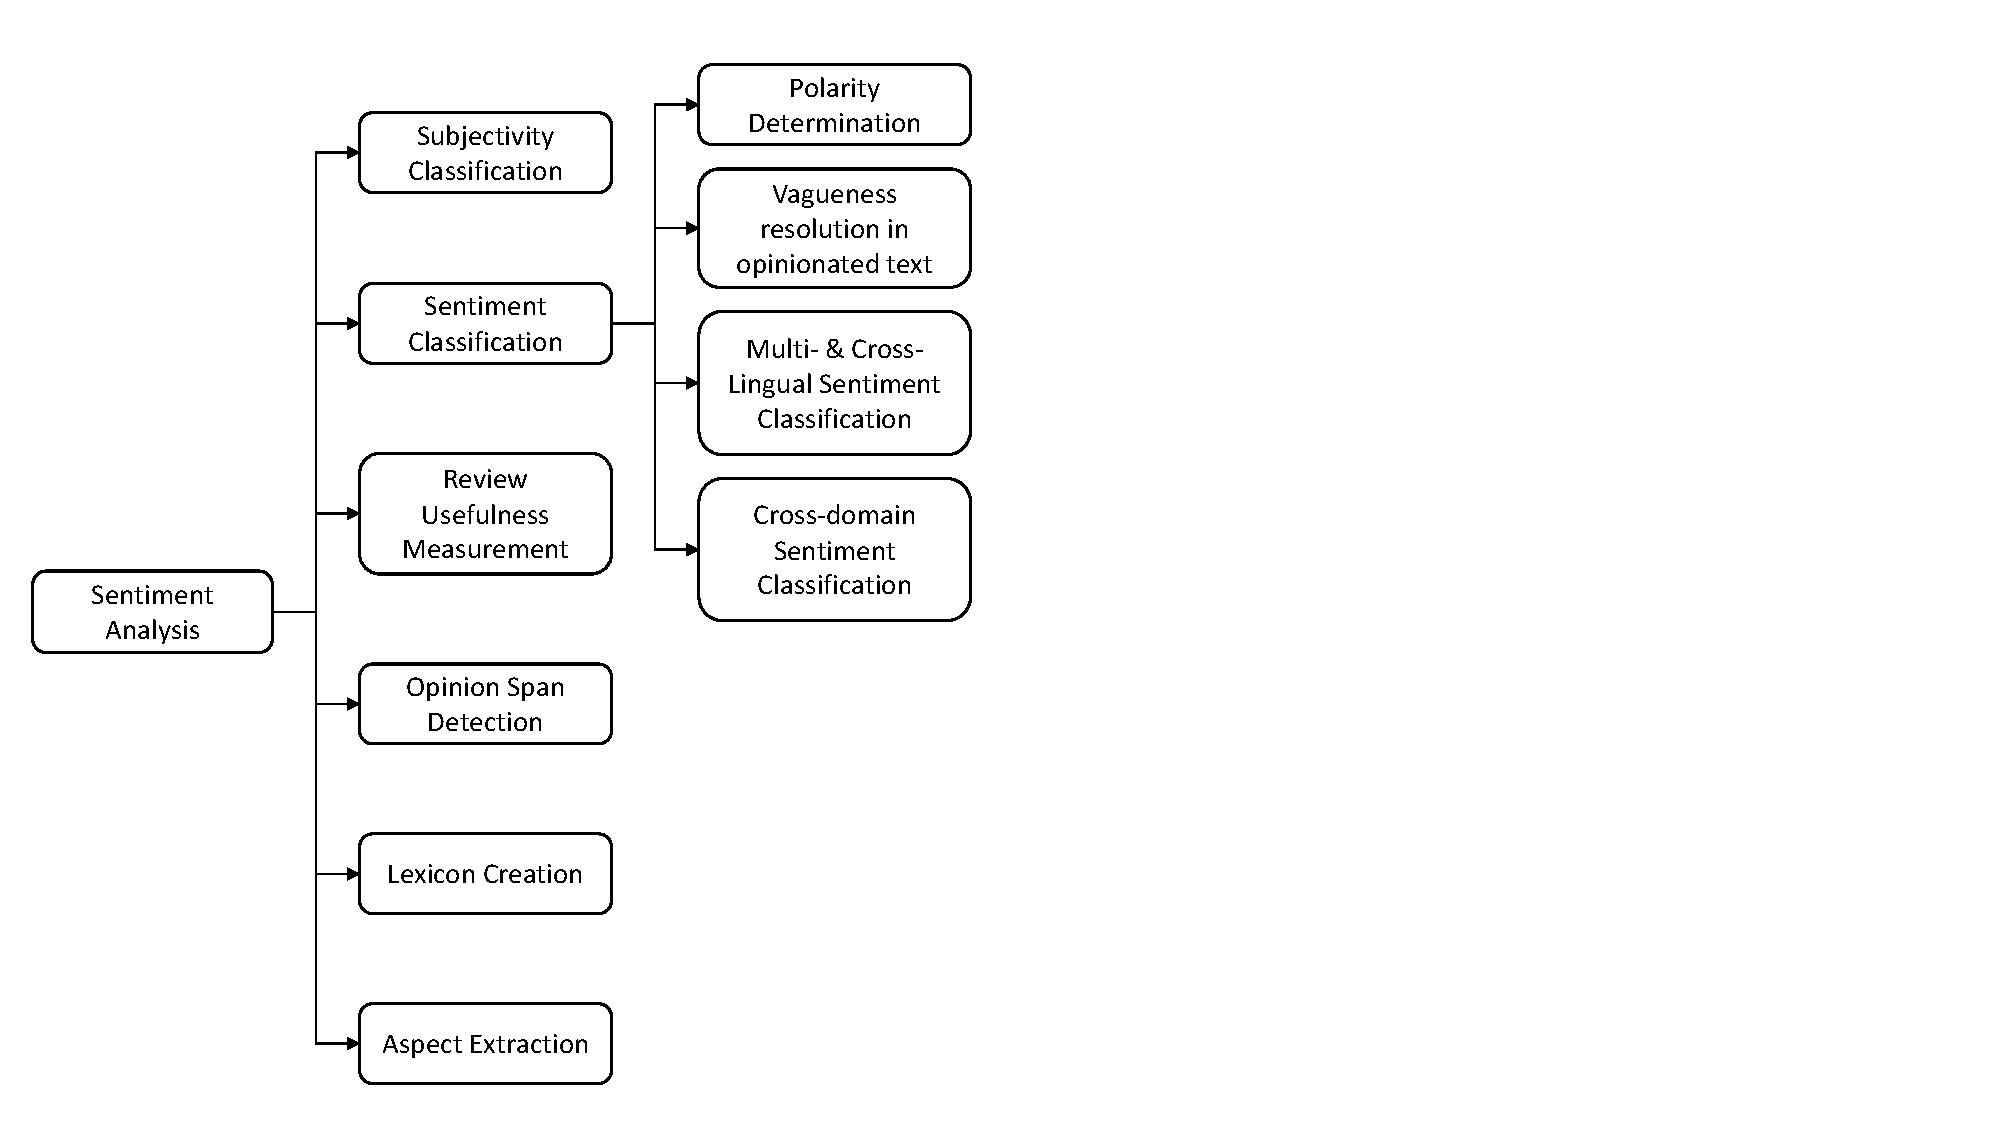
\includegraphics[width=1\textwidth]{figures/sentiment_analysis_tasks}
  \caption{Sentiment analysis tasks.}
  \label{fig:sentiment_analysis_tasks}
\end{figure}

Depending on the problem definition, different tasks have been defined related to sentiment analysis. According to \cite{ravi2015survey}, after the revision of more than three hundred papers related to this topic, the survey carried out concludes that the main tasks can be categorized as (a) subjectivity classification, (b) sentiment classification, (c) review usefulness measurement, (d) opinion spam detection, (e) lexicon creation and (f) aspect extraction, as shown in the figure \ref{fig:sentiment_analysis_tasks}. 

\subsubsection{Subjectivity classification}
\label{subsubsection:subject_classification}

According to \cite{montoyo2012subjectivity}, subjectivity classification aims to determine the "private state" of the author of a text. The Subjectivity analysis is the process of distinguish objective language from the opinion oriented. Even though there is much less literature about this field compared to other \acrshort{sa} task, it has proven to be more difficult than determine the measuring the polarity of a document and, thus, improvements achieved in this field will positively impact on sentiment classification.

\subsubsection{Sentiment classification}
\label{subsubsection:sentiment_classification}

Sentiment classification consist in determine the orientation of a sentiment of a given text into two or more classes. This classification has been performed in multiple classes, such as, binary (positive or negative), ternary (positive, neutral and negative), n-ary, \cite{nakov2016semeval}, among others.

\subsubsection{Review usefulness measurement}
\label{subsubsection:review_usefulness_measurement}

TODO

\subsubsection{Opinion spam detection}
\label{subsubsection:opinion_spam_detection}

TODO

\subsubsection{Lexicon creation}
\label{subsubsection:lexicon_creation}

TODO

\subsubsection{Aspect extraction}
\label{subsubsection:aspect_extraction}

TODO

To solve all these problems in the most efficient way, multiple approaches have been conducted, such as \cite{tripathy2016classification} ; \cite{mullen2004sentiment} or \cite{pouransari2014deep}. The figure \ref{fig:sentiment_analysis_approaches} illustrates which techniques have been used for each previously named categories.

\begin{figure}[!htp]
  \center
  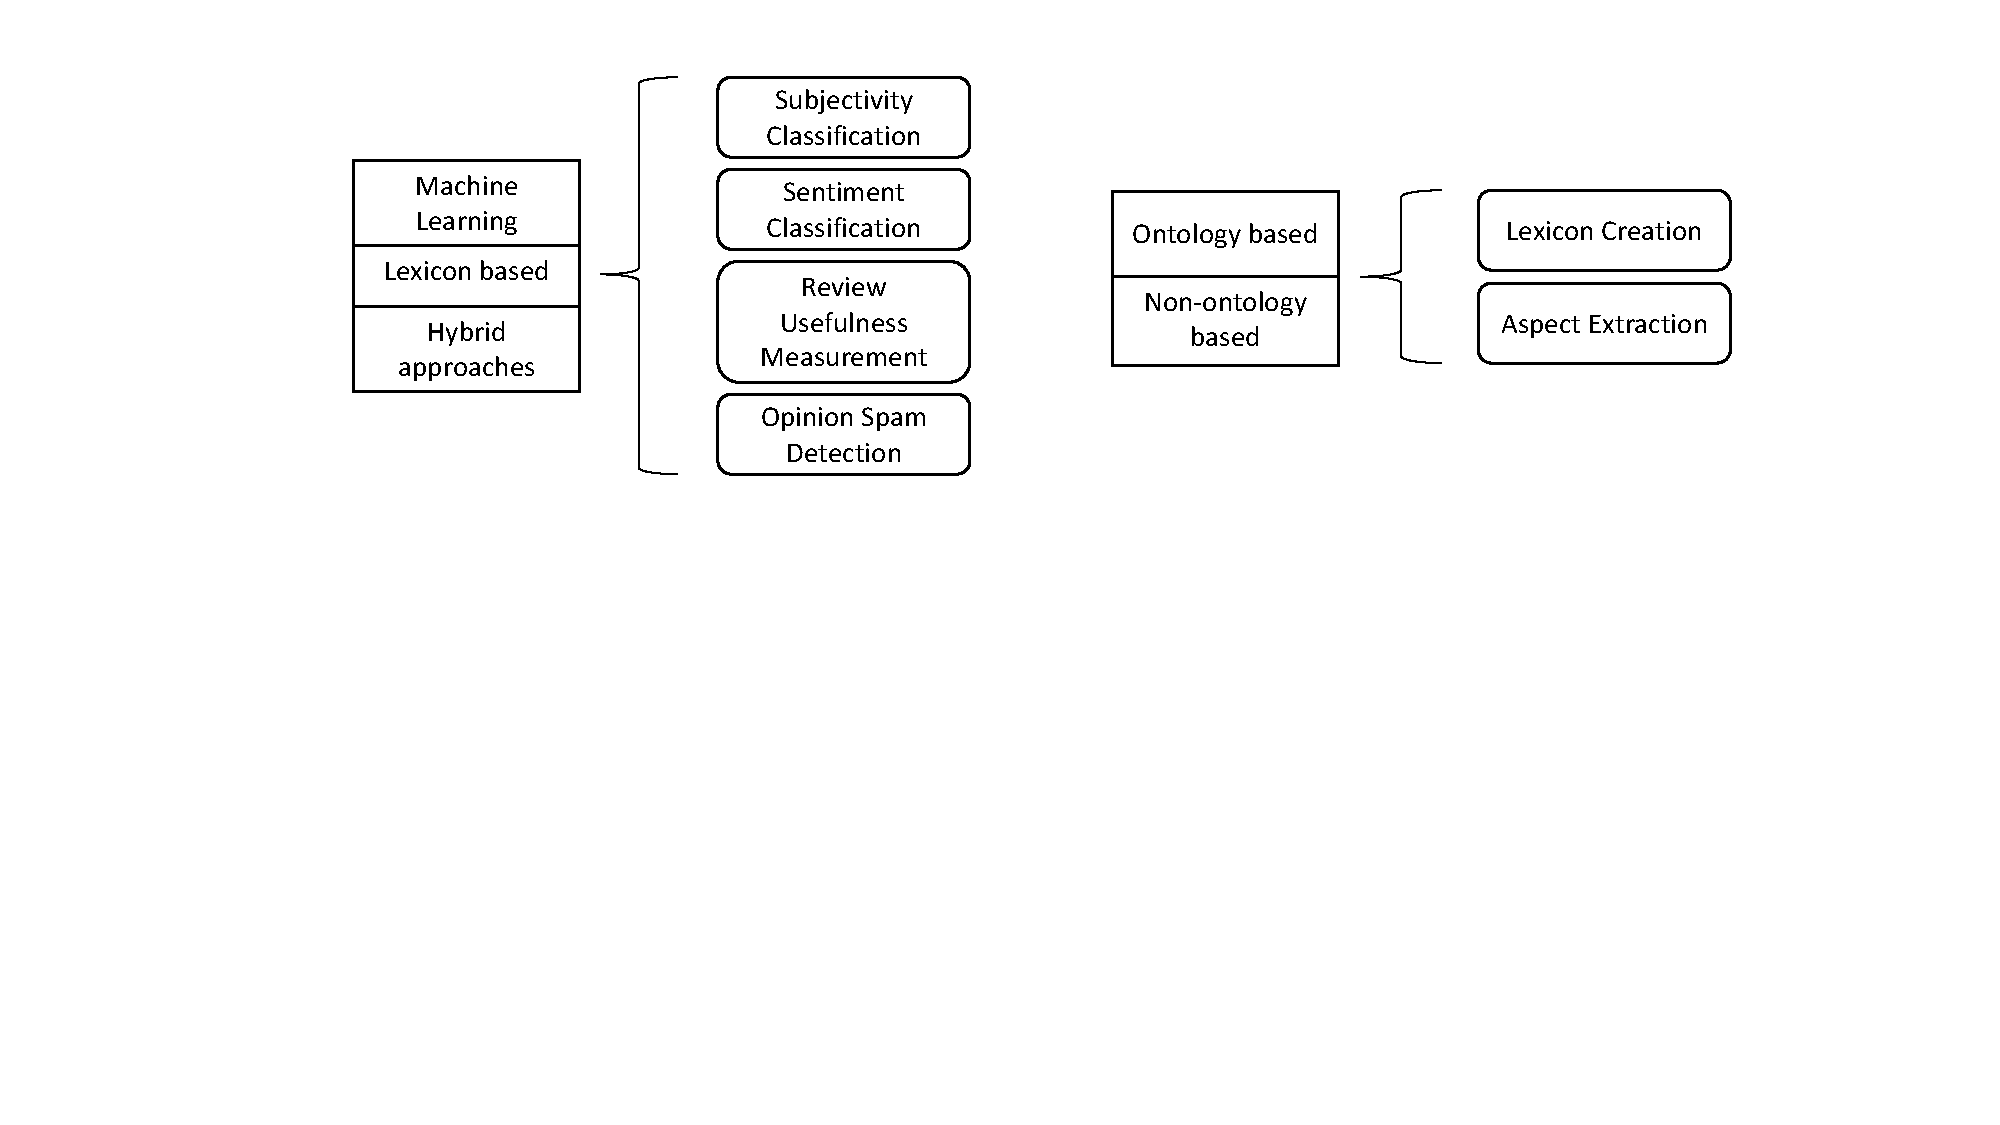
\includegraphics[width=0.9\textwidth]{figures/sentiment_analysis_approaches}
  \caption{Sentiment analysis approaches for each task.}
  \label{fig:sentiment_analysis_approaches}
\end{figure}

\FloatBarrier

\subsection{Techniques}
\label{subsec:sentiment_analysis_techniques}

TODO\cite{thakkar2015approaches}

\begin{figure}[!htp]
  \center
  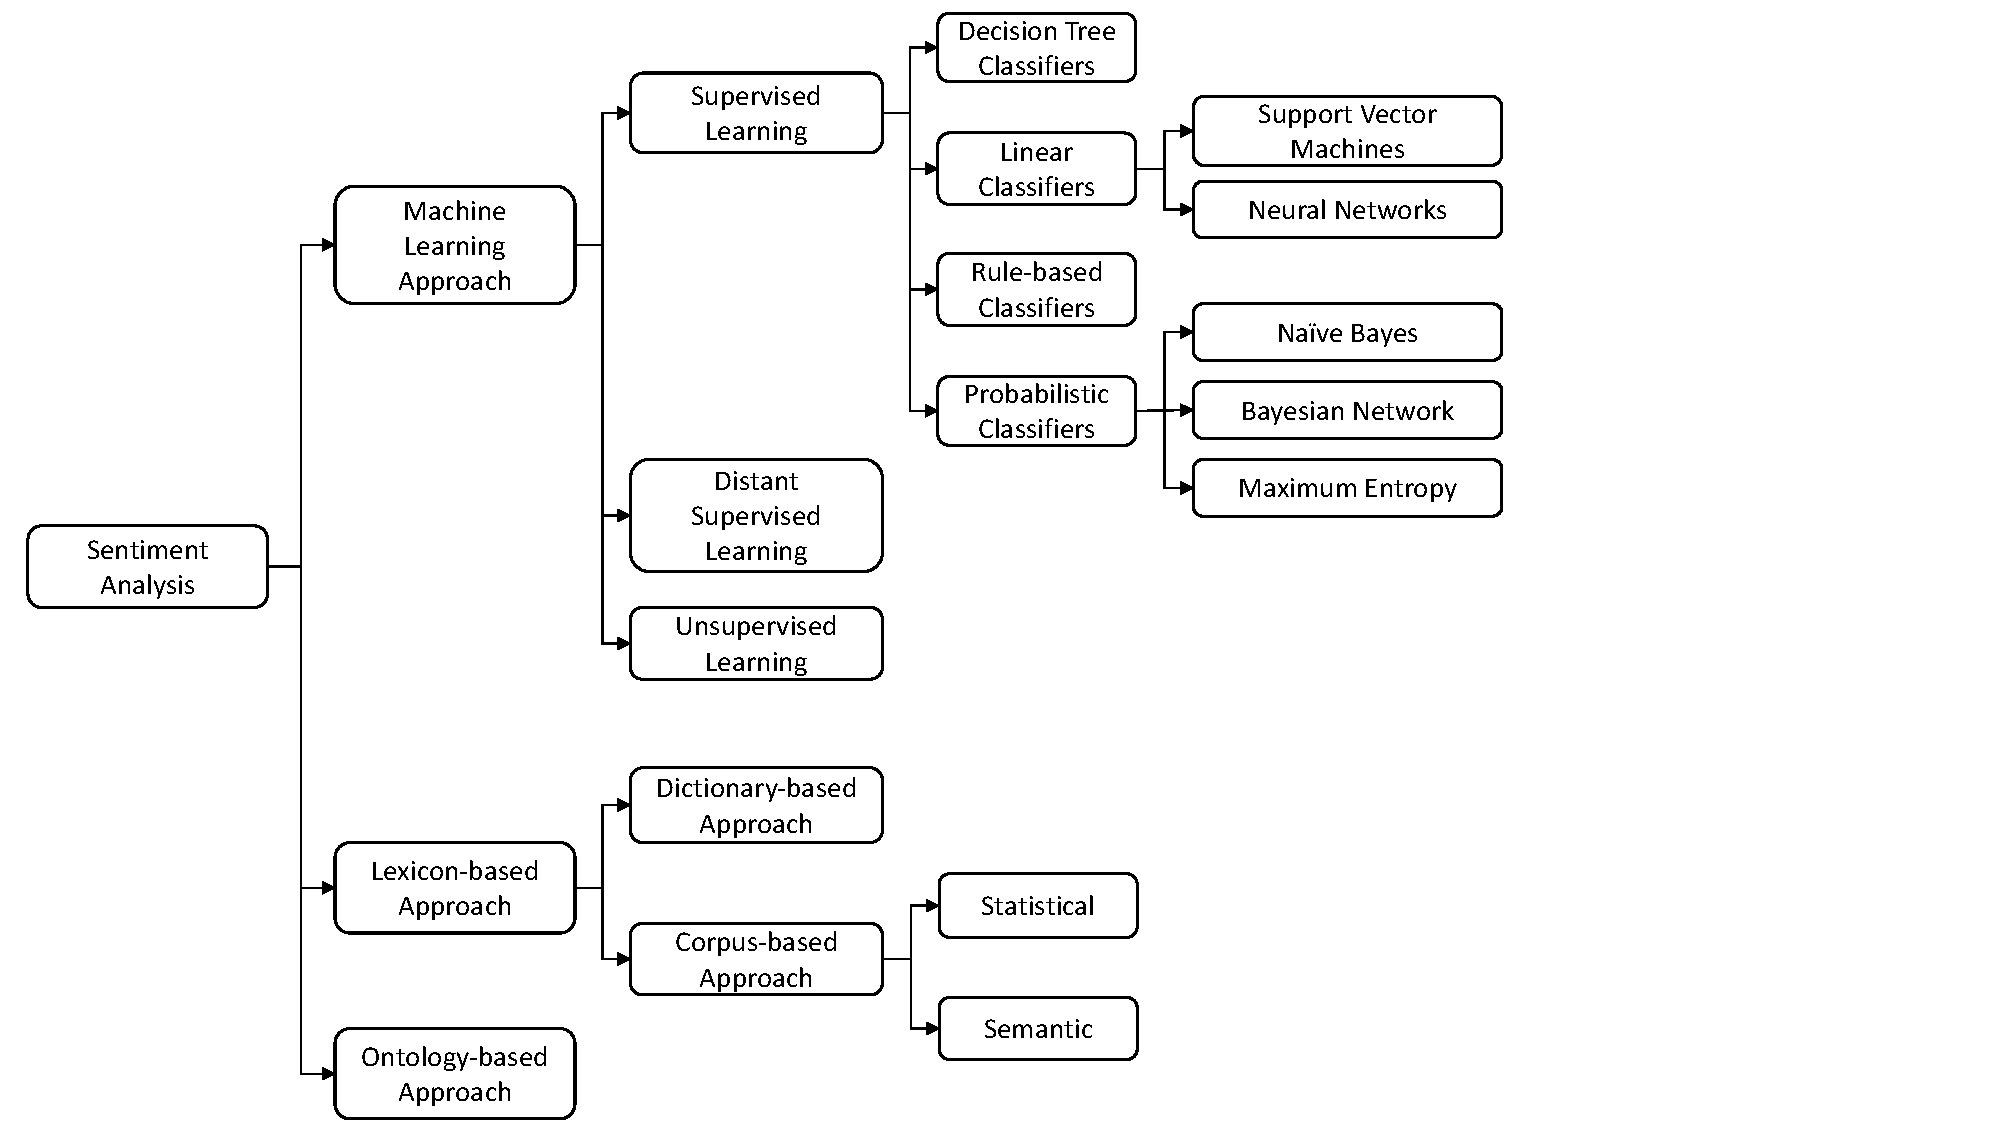
\includegraphics[width=1\textwidth]{figures/sentiment_analysis_techniques}
  \caption{Sentiment analysis techniques\cite{medhat2014sentiment}.}
  \label{fig:sentiment_analysis_techniques}
\end{figure}
% !TeX root = repressed-anger.tex

\section{Emotion Detection}
\label{sec:emotion_detection}

Emotion detection has been always a important field of study in neuroscience and psychology. Several experiments have been conducted to recognize emotions from face expressions, voice and body gestures, such in \cite{bassili1979emotion}; \cite{banziger2009emotion} and \cite{gunes2007bi}. However, these features are not always available and thus, the detection of emotion from text has gain relevance during the last decade.

Emotion detection from text documents is closely related to \acrshort{sa}. As explained in \ref{subsubsection:sentiment_classification}, sentiment classification task consists on determine the polarity of a given text into two or more classes. Emotion detection also fits this description, since this field of study is conducted by classifying a given document into predefined emotion labels. The definition of these labels are based on previously presented emotion models, which consist on application psychological and neuroscientific theories to represent emotions. One of the first model defined was proposed by Paul Ekman, on 1972, composed by six basic emotions, \textit{``happiness, sadness, fear, anger, surprise and disgust''}, and has been used in multiple face recognition systems that has become the base for emotion detection from text \cite{StevenEmotion2011Classification} as its definition has resulted to be the most semantically diverse \cite{bann2013conceptualisation}.

\begin{figure}[!htp]
  \center
  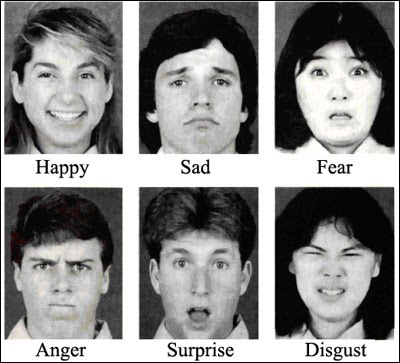
\includegraphics[width=0.67\textwidth]{figures/emotions_ekman}
  \caption{Ekamn's basic emotions, image extracted from Expressions, Emotions and Emblems, Google Sites.}
  \label{fig:ekman_basic_emotions}
\end{figure}

Since then, more interpretations have been made regarding the representation of the emotions as shown in \cite{cambria2012hourglass}. Ekman himself added his list 11 new emotions stating that not all of them could be represented by facial expressions. In 1980, Robert Plutchik created another bi-dimensional model (see figure \ref{fig:plutchik-wheeel}) known as wheel of emotions that defined eight basic bipolar emotions with different levels of intensification and could be combined among them. \acrfull{occ} designed in 1988 a model in which emotions were driven by an agent, based on the premise that \textit{``emotions are not themselves linguistic things, but the most readily available non phenomenal access we have to them is through language''} \cite{binali2010computational}. The model included 22 emotion categories that aimed to \textit{``model humans in general''} \cite{binali2010computational}. \acrshort{occ} enables the study of emotions as classes that share the same feeling, instead of specific words, proving that this \textit{``is a theory of emotions and not a theory of the language of emotions''} \cite{binali2010computational}. For more information, authors of \cite{binali2012emotion} analyze the state of art of the emotion models and the techniques used to generate them.

\begin{figure}[!htp]
  \center
  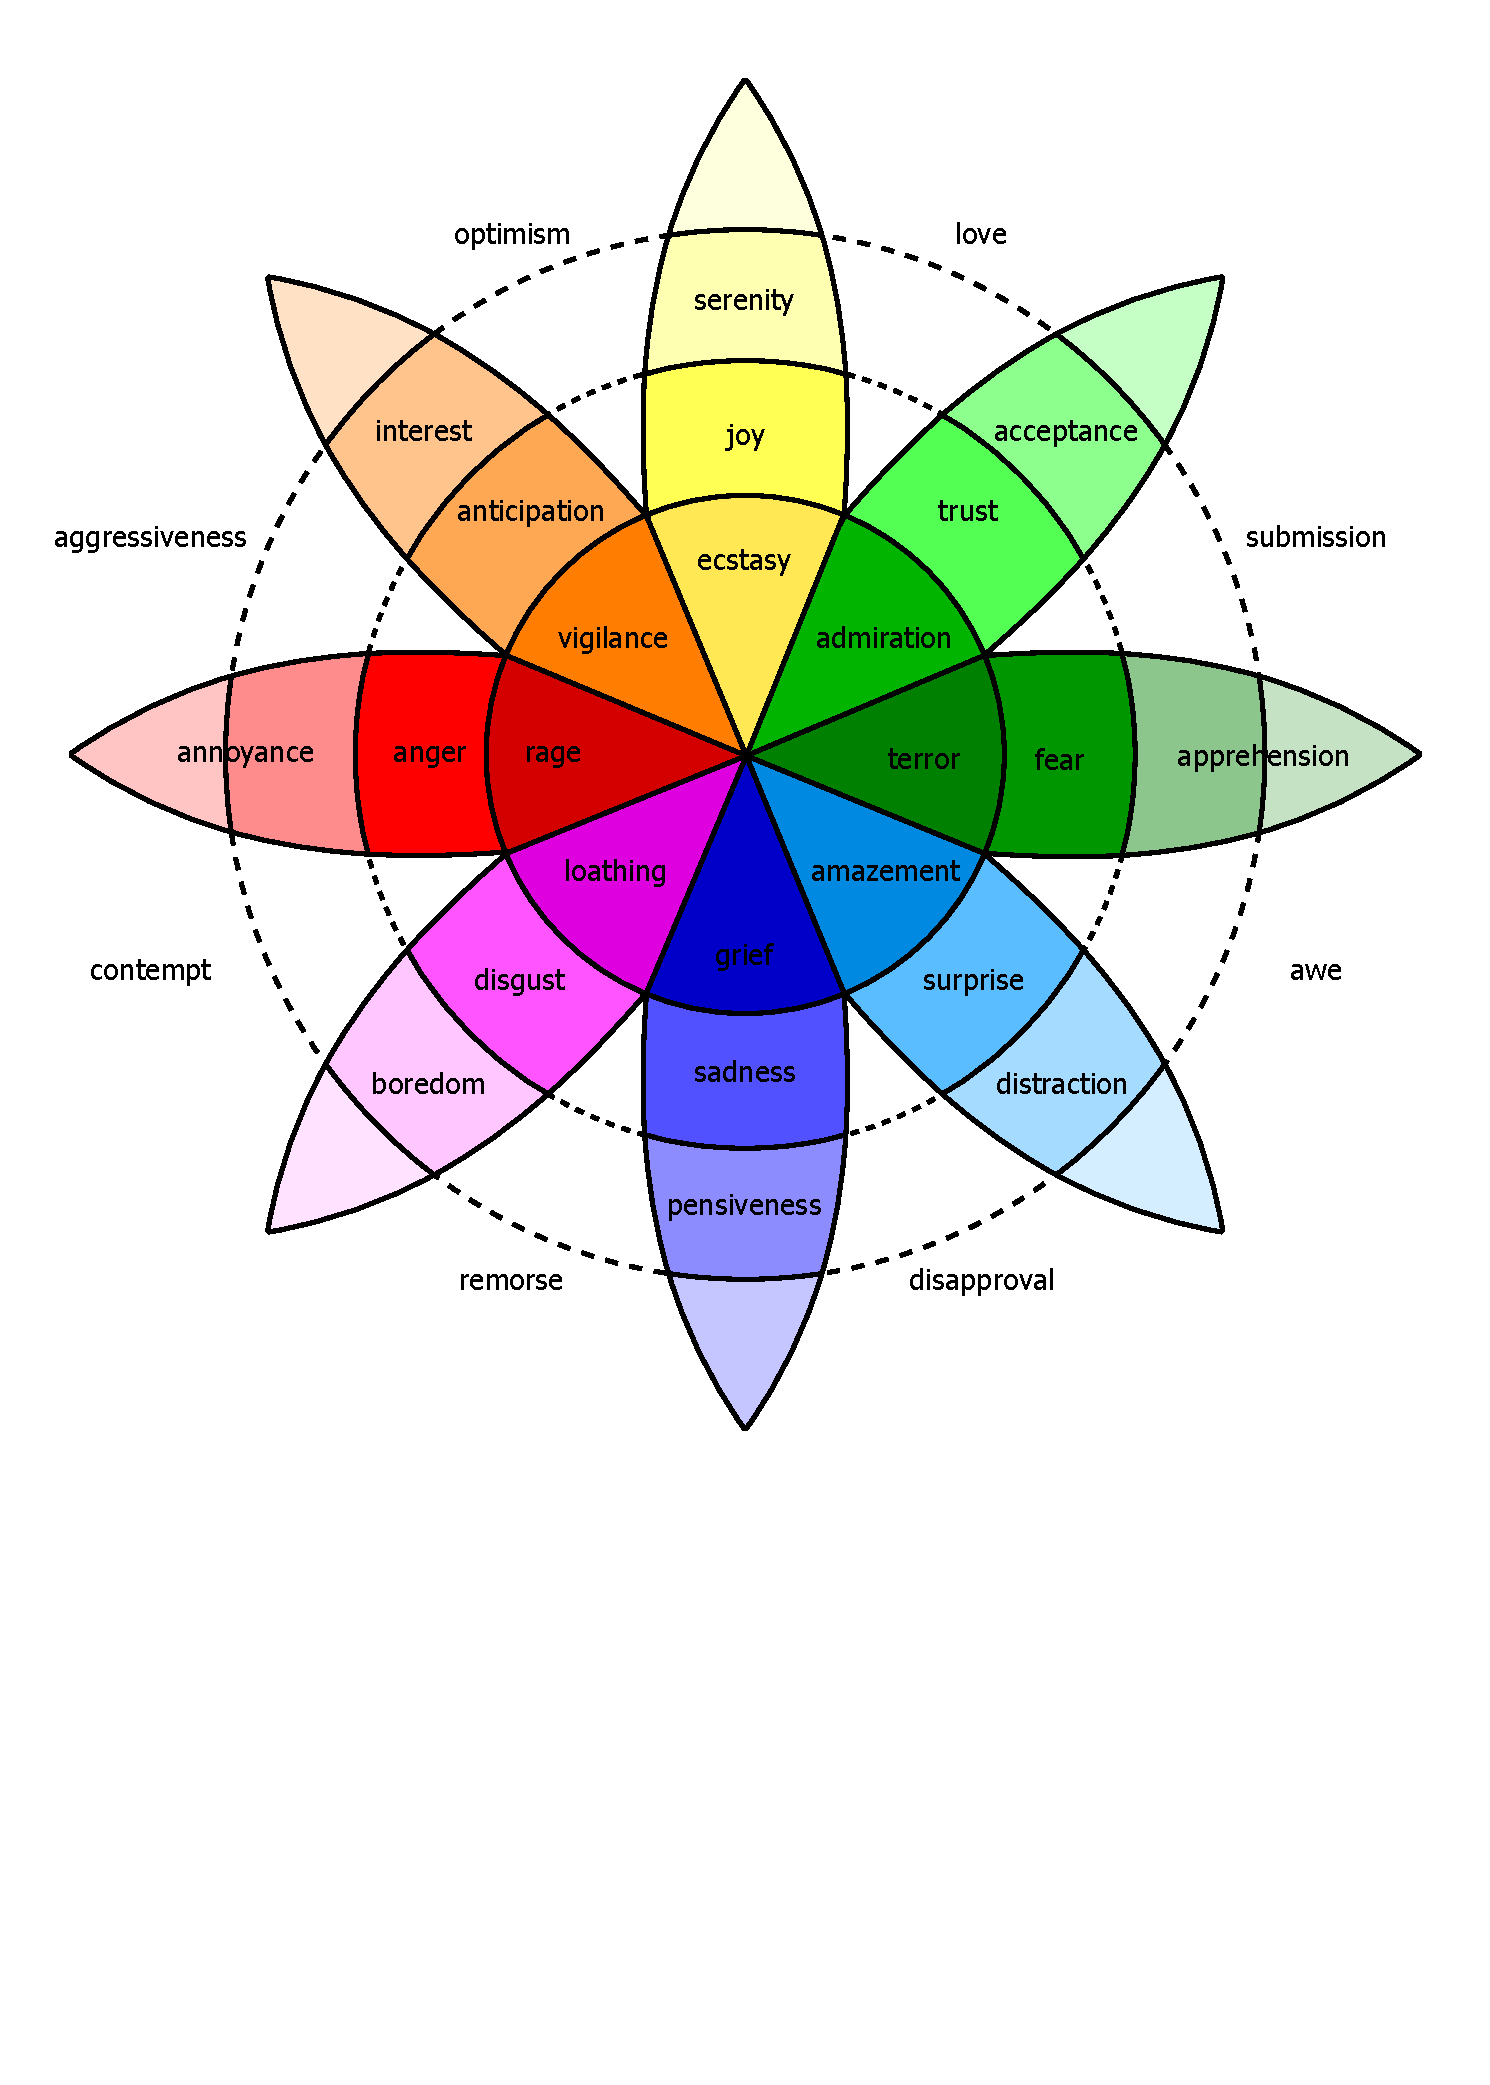
\includegraphics[width=0.67\textwidth]{figures/plutchik-wheel}
  \caption{Plutchik's emotion wheel, image extracted from Wikipedia's public domain.}
  \label{fig:plutchik-wheeel}
\end{figure}

Emotion classification tasks shares the same principles as \acrshort{sa}, and thus, the techniques used are mainly \acrshort{ml}, lexicon-based and hybrid approaches previously explained in section \ref{subsec:sentiment_analysis_techniques}.
% !TeX root = repressed-anger.tex

\section{Previous Work}
\label{sec:previous_work}

The study of anger and its management has been studied since ancient times. According to \acrfull{apa}, anger is \textit{``an emotion characterized by antagonism toward someone or something you feel has deliberately done you wrong''} \cite{angerAPA}. Anger is a normal emotion all human experience. Modern psychologists have studied the health effects that may derivate from anger suppression, such as shown in \cite{kemp1995anger} and \cite{hall1899study}, linking it to a more extremist and sarcastic personality. This research aims to find the answer to the question: \textit{``Can the repressed anger be detected in text?''}. Based on the definition of personality of a subject that has experienced repressed anger, the problem formulation has been simplified into finding negative messages influenced by the anger that is covered by a layer of sarcasm. The following subsections present a brief summary of the research conducted in the detection of anger and sarcasm.

\subsection{Anger}
\label{subsec:anger}

As explained in section \ref{sec:emotion_detection}, the increase of the usage of social media and computational viability to process all the publicly available data has enable the detection of emotions from text. However, as there is not literature that focuses on anger emotion, this section will briefly enunciate the approaches researched to classify emotions that contain anger as target label.

In 2007 during international workshop of evaluations of computational semantics analysis system, known as SemEval \cite{SemEvalPortal}, a task that analyzed the affective text was presented, in which the participants had to calculate the the valence and emotional class of news titles. Three groups participated in the emotion classification subtask: SWAT, UA and UPAR7. 

The system proposed by SWAT was based on unigram trained model supervised learning. In addition to the emotion label target given this group perform a synonym expansion of these keywords from Roget Thesaurus English book. The training of the system was performed by combining the development data provided by the SemEval task organizers plus a set of 1000 headlines that was annotated from the group.

UPAR7 developed a linguistic rule-based system approach. The first step was to pre-process the data by un-capitalize the common words. Then, each word was rated separately with each emotion target label. 

In order to determine the type of emotion in the headline, UA group collected statistics from three web search engines to calculate the distribution of nouns, verbs, adjectives and adverbs of the headline. The emotion scores were obtained through \acrfull{pmi}.

The F1-score obtained by SWAT, UA and UPAR7 for anger sentiment was 7.06, 16.03 and 3.02 respectively (results multiplied by 100) \cite{strapparava2007semeval}.

Authors in \cite{strapparava2008learning} implemented five system for emotion analysis based on knowledge based emotion annotation and corpus based emotion annotation: \acrshort{wn}-affect presence, \acrshort{lsa} single word, \acrshort{lsa} emotion synset, \acrshort{lsa} all emotion words and \acrshort{nb} trained on blogs. For anger annotation, the proposed system scored a F1-score of 16.77 (results multiplied by 100), outperforming the system proposed by UA in SemEval for anger annotation.

Kirk Roberts et al. developed a system composed of seven \acrshort{svm} classifiers, one for each Ekman's sentiment basic emotion plus anticipation. The Features selected as input for the binary classifier where: unigrams, bigrams, trigrams, presence of interrogation or exclamation mark, \acrlong{wn} synsets, \acrshort{wn} hypernyms, \acrlong{lda} topic scores and high \acrshort{pmi} unigrams (significant words). The anger classifier used unigrams, synsets, topis and significant words, scoring a F1-score of 0.642 \cite{roberts2012empatweet}.

Chew-Yean Yam posted at Microsoft developer Blog an example of emotion classification using \acrfull{dl} techniques. The corpus was collected by using Amazon's Mechanical Turk to perform a \acrfull{hit} to manually annotate the data, obtaining a total of 784,349 samples of informal short English messages classified as five classes, anger, sadness, fear, happiness and excitement. The \acrshort{dl} architecture is described as a \acrfull{nn} with five out nodes, three hidden layers, that contain 5, 25 and 125 nodes respectively. The loss function selected was cross entropy with a stochastic gradient descent optimization algorithm. The learning rate was set to 0.001. The maximum training iteration was set to 100 with a greedy pre-trainer type executed though-out 25 epochs. The anger classifier in this system obtained a F1-score of 0.64958 \cite{microsoftEmotionAPI}.

\subsection{Irony and Sarcasm}
\label{subsec:irony_sarcasm}

Sarcasm, also referred as verbal irony \cite{giora2013negation}; \cite{giora2015defaultness} and \cite{giora2015default}, is defined as cutting remark to express contempt or ridicule according the free dictionary \cite{sarcasmFreeDictionary}. Based on the literature, the boundaries of irony and sarcasm are fuzzy \cite{bosco2013developing}, as some authors consider irony as global term that includes sarcasm \cite{gibbs1991psychological}, \cite{wilson2006pragmatics} and \cite{kreuz1993empirical} and others analyze the differences between both \cite{filatova2012irony}.

Authors in \cite{joshi2016automatic} conduct a survey of the approaches used to detect sarcasm. Mainly three approaches have been proposed: rule-based, statistical approaches and \acrlong{dl} approaches.

In 2009, Paula Carvalho et al. analyzed the detection of Portuguese irony by using pattern matching rules, such as diminutive forms, interjections, verb morphology, heavy punctuation, quotation marks, laughter expressions, among others. The proposed system classified the given sentences as ironic, not ironic, undecided and ambiguous. They concluded that the best patters for irony recognition are quote and laugh patterns, obtaining an accuracy of 68.29\% and 85.40\% respectively \cite{carvalho2009clues}.

\cite{maynard2014cares} developed in 2014 a rule based system to classify sentences in which the presence of sarcasm was known by analyzing hashtags on Twitter. Based on the premise that if the hashtag does not agree with the rest of the tweet the sentence is classified as sarcastic and by re-tokenizing hashtashs to split concatenated tokens, the classifier obtained a F1-score of 91.03 (result multiplied by 100).

Two important aspects must be pointed out regarding statistical approaches: the features used and the selected learning algorithms. Aditya Joshi et al.'s survey states that even though \textit{``a variety of classifiers have been experimented for sarcasm detection most of the work conducted relies on \acrshort{svm}''} \cite{joshi2016automatic}.

Authors in \cite{davidov2010semi} proposed a system that classified Twitter and Amazon documents by employing semi-supervised techniques. The dataset was composed of 5.9 million unique tweets that contained the \#sarcasm hashtag, which were pre-processed by removing any link appearance, users mentions and hashtags and replaced them by proper identification tags. The system relied on features such as \acrfullpl{hfw}, \acrfullpl{cw}, punctuation based features to create single entry feature vectors. The classification output was defined as a number from 1 to 5 to measure the presence of sarcasm in the given text and performed with a \acrfull{knn}-like strategy \cite{davidov2010enhanced}. To evaluate the system 5-fold cross validation was employed. The experiment that best performed used all the listed features and obtained a F1-score of 0.545 on Twitter messages and 0.827 in Amazon reviews.

In 2012, Reyes et al. introduced the following features for irony detection: n-grams, \acrfull{pos} n-grams, funny profiling, positive/negative profiling, affective profiling and pleasantness profiling. \acrshort{nb}, \acrshort{svm} and \acrfull{dt} classifiers were evaluated by comaparing positive sets against three negative subsets, begin \acrshort{svm} the learning algorithm that scored the highest in two out of the three subsets with a F1-score of 0.747 and 0.891 respectively \cite{reyes2012making}. In 2013, they explored the use of skip-gram and character n-gram-based features for detecting irony representativeness and relevance with the Toyota case study. Dividing the tweets into three levels of representativeness the proposed model obtained a 0.66 F1-score on the third level \cite{reyes2013multidimensional}.

Regarding \acrshort{dl}, is a technology that is gaining popularity among researchers studying sarcasm and irony. Silvio Amir et al. in 2016 proposed a convolutional network-based system that learned content and context from user embeddings, achieving a 2\% improve in absolute accuracy compared to the Bamman and Smith's 2015 baseline system \cite{amir2016modelling}. 

Authors in \cite{ghosh2016fracking} proposed a system that combined \acrfull{cnn}, \acrfull{lstm} and \acrfull{dnn}. They compare the approached system against recursive \acrshort{svm} and other datasets, stating that their architecture obtains better F1-score than previous \acrshort{dl} solutions, with a F1-score of 0.901.

Main activity: Paper reading

Introduction to Sentiment Analysis.
Relevant International Workshop found: SemEval
→ Datasets repositories: Twitter as corpus, Amazon products reviews…
→ Dataset labeling: CrowdFlower, Amazon Mechanical Turk.
→ Word embedding: Word2vec, GloVe.
→ Text classification features: N-grams based on Sentiment lexicon…
→ Learning Methods: Supervised, Unsupervised, Distant…
→ Deep Learning techniques: Convolutional NN, Recurrent NN, Deep Autoencoders…
→ Classifiers: “Bag of Words”, Naive Bayes, Logistic Regression, SVM, NN, Clustering…
→ Accuracy evaluation: Precision, Recall, F1-Score, Cross-validation…
→ Trends: Best scoring teams used Deep Learning techniques.

Differences between Sentiment and Emotion Analysis

SemEval works on sentiment analysis, which focuses on binary or multiclass classification, being Positive, Neutral and Negative the most common one.
This means:
 None of the SemEval preprocessed datasets are valid for me. (Raw data may work for manual annotation)
 The need of procedure adaptation to fit my research domain.
E.g. Use Emotion lexicon, such as EmoLex or LIWC, instead of  those related to Sentiment.
Need to focus the research on discover word features that help to classify anger in texts.
E.g. Heavy Punctuation, Quotation Marks, Emoticons; Unigrams, among others.

Next week work: Deep reading and prepare a Playground with small sample data.

Read fundamental theory about classifiers such as SVN, Bayesian, KNN, Decision Tree.
Urge test what has been learned in order to set the basic knowledge.
→ Download and test WEKA’s basic functionalities for educational and research purpose. (Includes a No-Code-GUI, which makes it user friendly for initial testings)
→ Use scikit-learn for following iterations of the classifier (More modern algorithms, better memory management, Python development environment...)
Further reading about Emotion classification techniques and investigate about repressed anger in English texts. 
Multiclass angry classification?

Future work: Deep Learning

Depending on the generated dataset (size and labeled/unlabeled) the project could opt for a DL based classifier.
Could score better results in the benchmarking.
→ To gather large amount of data for each class is compulsory solve the overfitting problem. (Detection and prevention by using Cross-validation)
→ If the dataset is not completely labeled weakly (distant) supervised learning could be applied.
→ Theano and Keras have proved a DL frameworks to perform well.

% !TeX root = repressed-anger.tex

\section{Classification Techniques}
\label{sec:algorithms}

The aim of this section has two purposes. The first one, is to make an introduction of the basic concepts of classification, which is essential for the detection of repressed anger as the solution proposed has been defined as a classification problem. The second one, is to explain how the algorithms used in this study work.

\subsection{Fundamentals of Classification}

According to \cite{voznika2007data}, classification can be defined as the task of predicting an outcome from a given input. This outcome is produced by the process of mapping a group of characteristics present in the input to a certain category. In other words, it consists in assigning objects (the input) to one of several predefined classes (the outcome) \cite{pang2006introduction}. Examples of classification can be found in everyday life, such as e-mail spam detection, news classifiers, \acrfull{ocr}, animal kingdom classification (see Figure \ref{fig:animal_classification}), among many others.

\begin{figure}[!htp]
  \center
  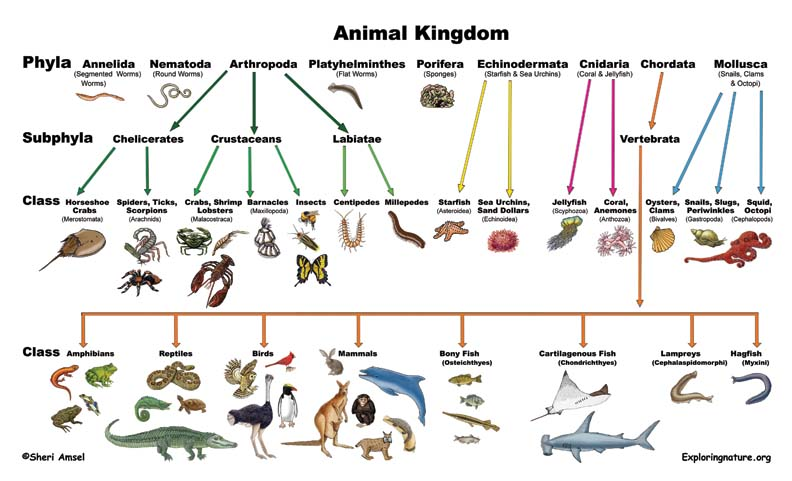
\includegraphics[width=0.85\textwidth]{figures/animal_classification}
  \caption{Classification of animals. The image is extracted from Exploring Nature.}
  \label{fig:animal_classification}
\end{figure}

\FloatBarrier

The input data for a classification task is composed by a collection of records, the dataset. In the same time, each record, also known as an instance, is composed by a set attributes. From all these attributes there is one considered special, which is called the target attribute or the class label. Regular attributes can be both discrete or continuous values. For the values signed for the class label, however, they must be discrete. This characteristic is what distinguishes classification form regression. Table \ref{tab:clasiffication_table} shows a sample dataset for animal classification into the following categories: amphibian, bird, fish or mammal.

\begin{table}[!htp]
\centering
\begin{tabular}{ |c|c|c|c|c|c|c|c| }
\hline
Common Name & Hair & Feathers & Eggs & Milk & Aquatic & Legs & Class Label \\ \hline
antelope & Yes & No & No & No & No & 4 & mammal \\ \hline
catfish & No & No & Yes & No & Yes & 0 & fish \\ \hline
dolphin & No & No & No & Yes & Yes & 0 & mammal \\ \hline
dove & No & Yes & Yes & No & No & 2 & bird \\ \hline
duck & No & Yes & Yes & No & Yes & 2 & bird \\ \hline
elephant & Yes & Yes & No & Yes & No & 4 & mammal \\ \hline
flamingo & Yes & Yes & Yes & No & No & 2 & bird \\ \hline
frog & No & No & Yes & No & Yes & 4 & amphibian \\ \hline
fruit bat & Yes & No & No & Yes & No & 2 & mammal \\ \hline
gull & No & Yes & Yes & No & Yes & 2 & bird \\ \hline
herring & No & No & Yes & No & Yes & 0 & fish \\ \hline
kiwi & No & No & Yes & No & No & 2 & bird \\ \hline
lark & No & Yes & Yes & No & No & 2 & bird \\ \hline
lynx & Yes & No & No & Yes & No & 4 & mammal \\ \hline
mole & Yes & No & No & Yes & No & 4 & mammal \\ \hline
mongoose & Yes & No & No & Yes & No & 4 & mammal \\ \hline
newt & No & No & Yes & No & Yes & 4 & amphibian \\
\hline
\end{tabular}
\caption{Animal kingdom dataset.}
\label{tab:clasiffication_table}
\end{table}

Tan Pang-Ning et al. propose a more mathematical definition of classification stating that it is the process of learning a target function $f$, also known as classification model, that maps each attribute set $x$ to one of the predefined class labels $y$.

\begin{figure}[!htp]
  \center
  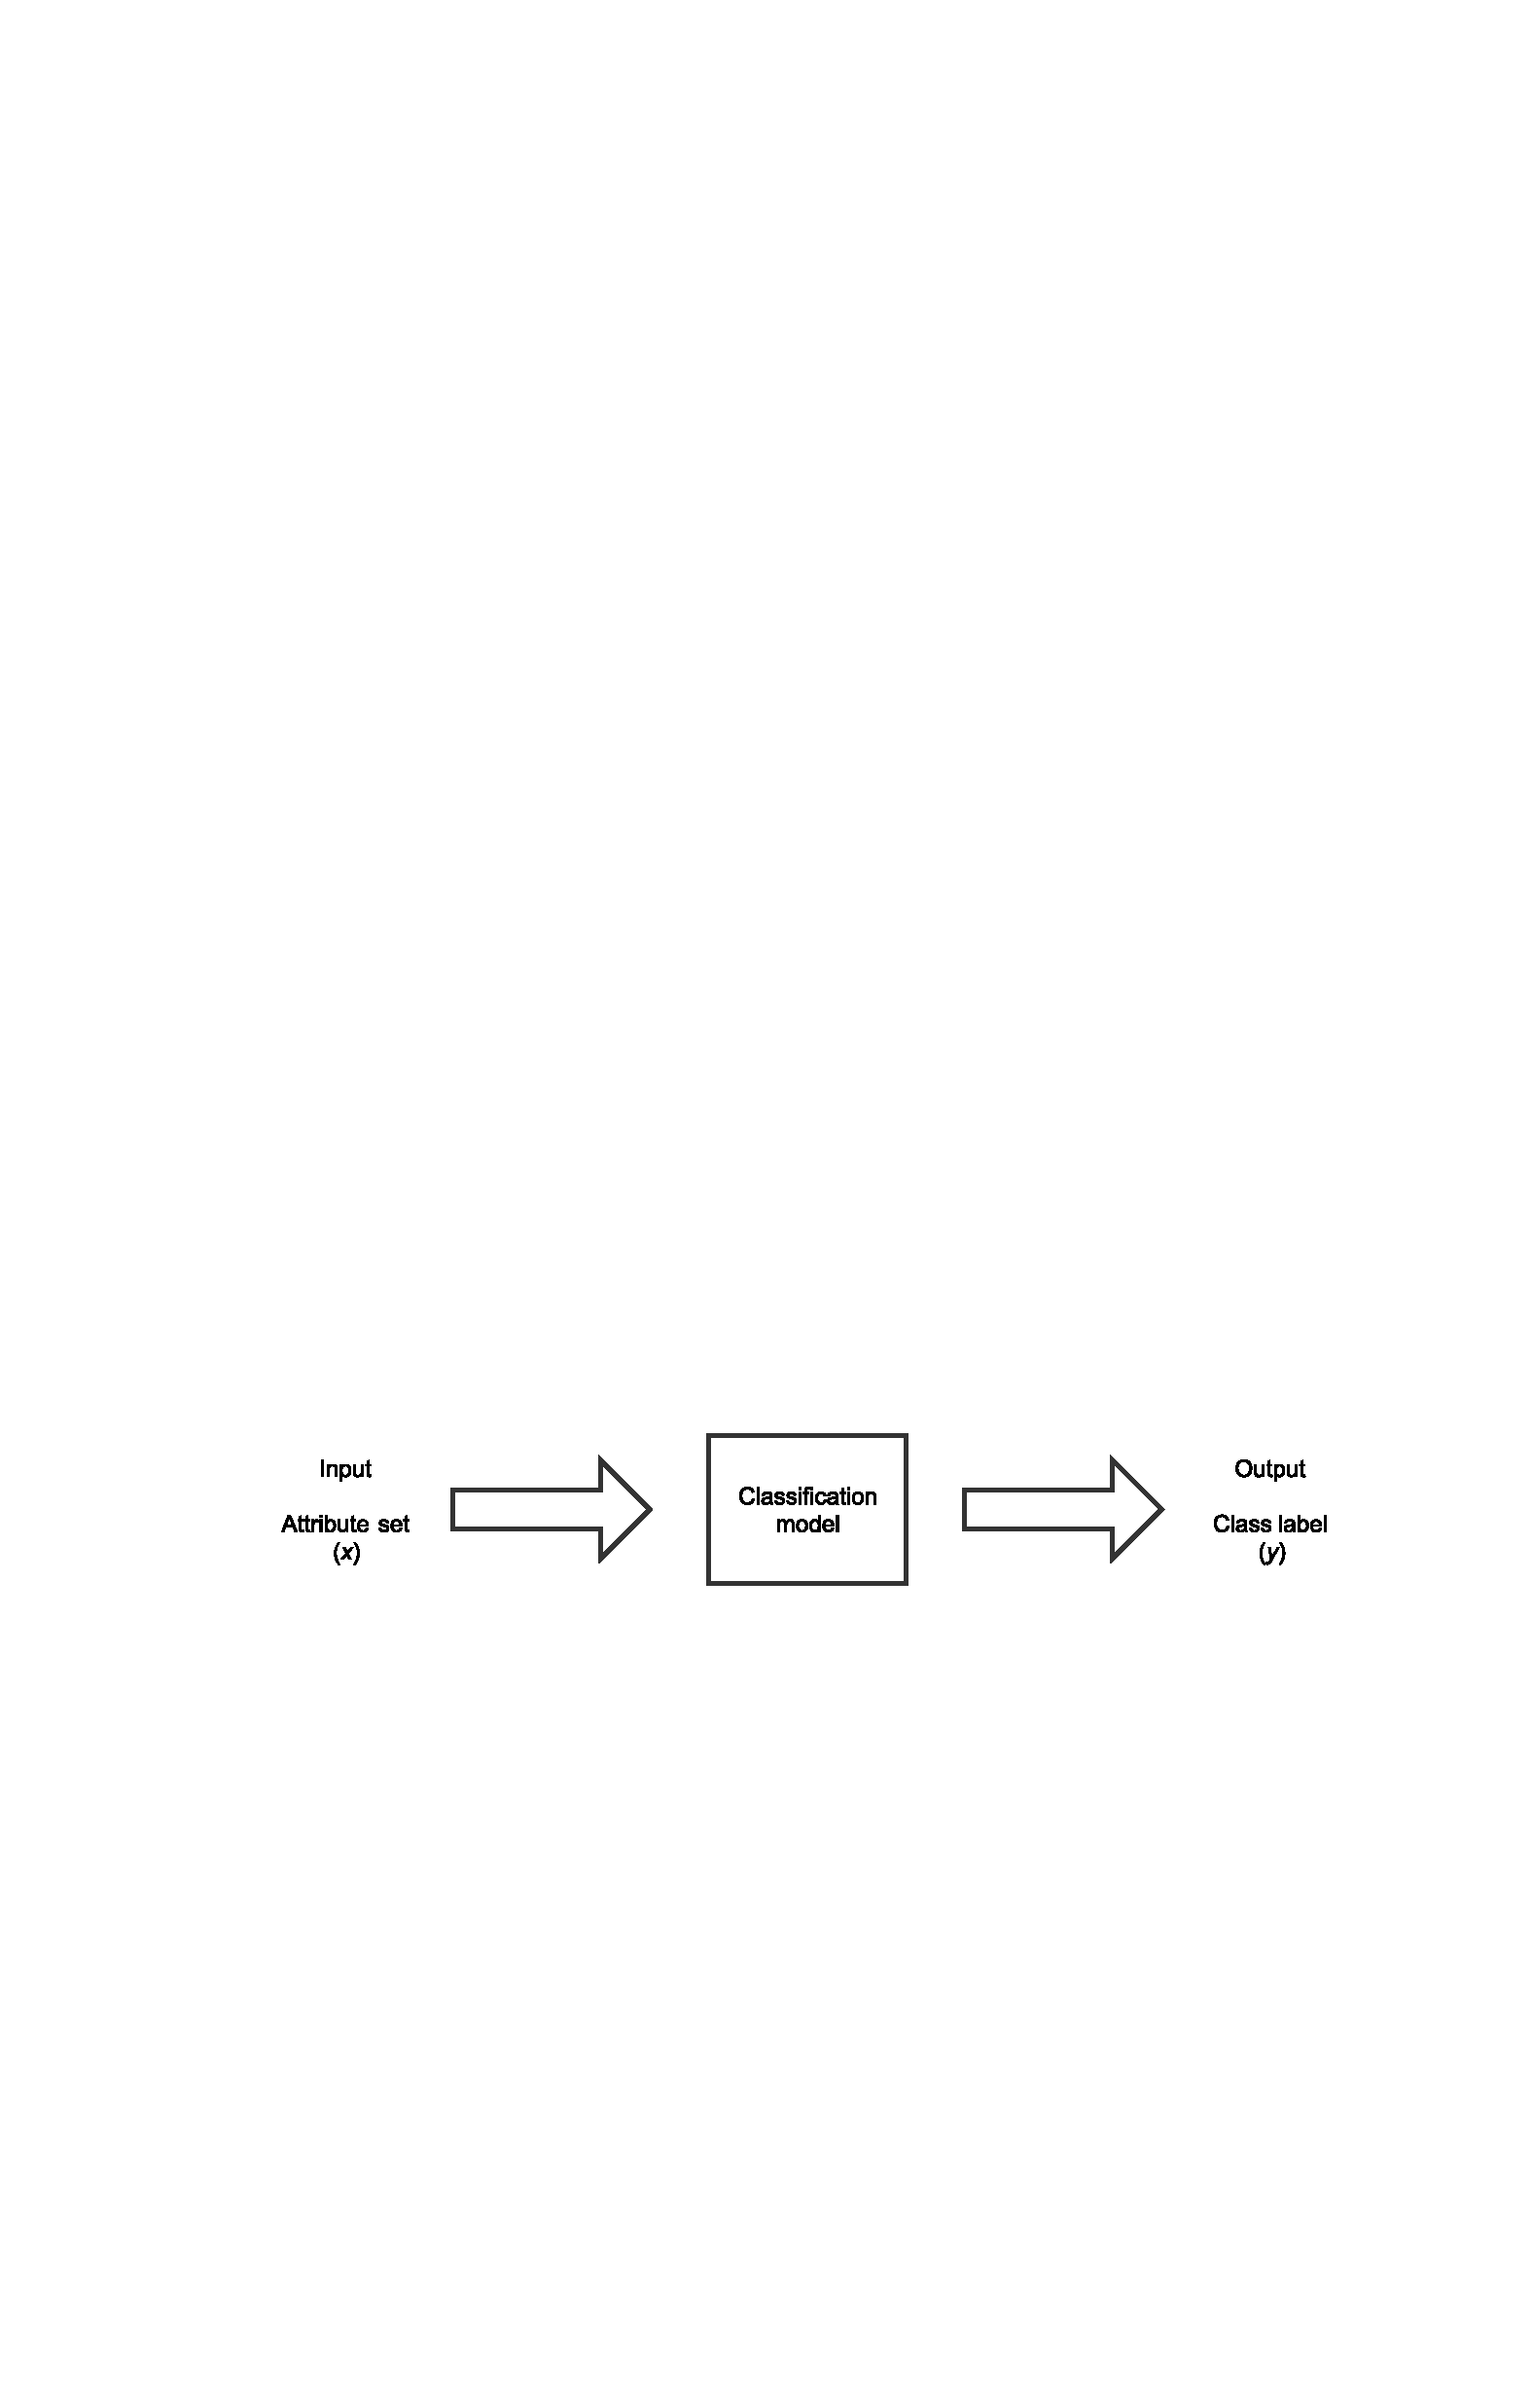
\includegraphics[width=\textwidth]{figures/classification}
  \caption{Classification as a task of mapping a set attributes $x$ into its fitting class label $y$.}
  \label{fig:classification_task}
\end{figure}

A classification model is useful for the following purposes \cite{pang2006introduction}:

\begin{itemize}
\item \textbf{Descriptive Modeling:} Since a classification model presents the main features of the data, it can serve as an explanatory tool to distinguish between instances of different categories \cite{madigan2002descriptive}.

\item \textbf{Predictive Modeling:} A classification model can also be used to predict the class label of an unknown new instance. As shown in Figure \ref{fig:classification_task}, a classification model can be represented as a black box that automatically assigns a class label to an instance by providing its attribute set.
\end{itemize}

It is important to remark that classification techniques perform their best when used for predicting or describing datasets which its class label is binary or nominal, Since they no consider properties such ordinality or the implicit order among the categories, they become ineffective with ordinal class labels \cite{frank2001simple}.

\subsection{General classification problem solving}
\label{general_classificartion_problem_solving}

For general classification problems solving, popular techniques consists on a process that starts with building classification models from a sample dataset \cite{witten2005data}. Each technique depends on a learning algorithm witch is in charge of generating the classification model. A good model should define the relationship between the input attribute set and its belonging category that suits the best. Therefore the model should be valid for both, the sample data used to generate the model and also for new unknown instances. Among popular classification techniques \acrfull{svm}, \acrfullpl{nn}, Naive Bayes or \acrfullpl{dt} can be found \cite{garje2016sentiment}.

\begin{figure}[!htp]
  \center
  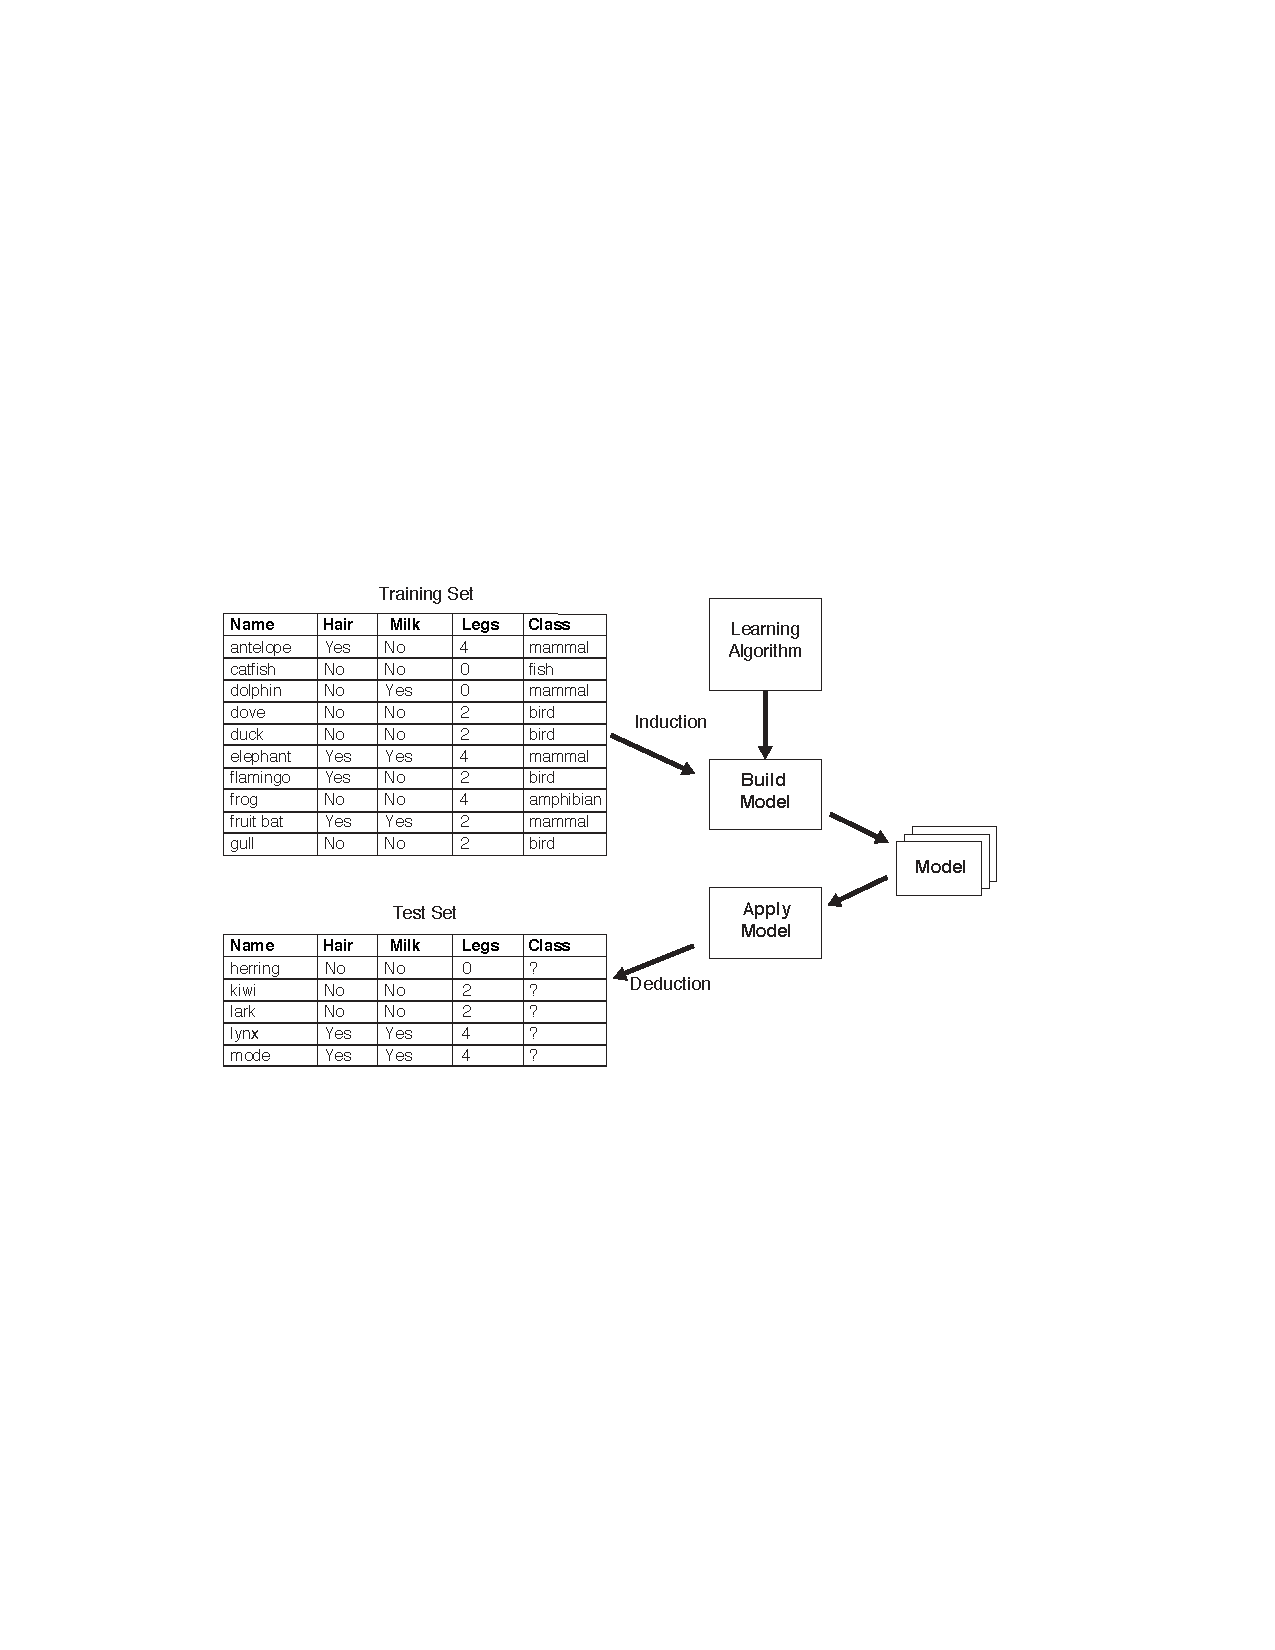
\includegraphics[width=0.85\textwidth]{figures/classification_problem_solving}
  \caption{General approach for classification model building and new instance category prediction.}
  \label{fig:classification_problem}
\end{figure}

As shown in the Figure \ref{fig:classification_problem}, to solve a classification problem a sample dataset must be provided as a training set. This sample is used to build the classification model according to the learning algorithm. After the model is built, it is applied to unlabeled dataset, also called the test set, to predict the categories of each instances of the records. To measure how good the model is, there is only need to count the number of instances have been correctly and incorrectly classified from the test set. Usually, to represent system's performance values, a confusion matrix is used \cite{hamilton2000confusion}. 


\begin{table}[!htp]
\centering
\begin{tabular}{ |c|c|c|c| }
\hline
\multicolumn{2}{|c|}{} & \multicolumn{2}{c|}{Predicted Class} \\
\hhline{~~--}
\multicolumn{2}{|c|}{} & $Class = Yes$ & $Class = No$ \\ \hline
\multirow{2}{*}{Actual Class} & $Class = Yes$ & a & b \\
\hhline{~---}
& $Class = No$ & c & d \\
\hline
\end{tabular}
\caption{Confusion matrix of a binary classification.}
\label{tab:confusion_matrix}
\end{table}

As a example, Table \ref{tab:confusion_matrix} represents the confusion matrix of a binary classification problem, in which the possible classes that can be assigned to a given instance are \textit{Yes} or \textit{No}. The values presented in this confusion matrix represents the counts of instances correctly and incorrectly classified as a means of model performance evaluation, being the diagonal of the table the instances classified correctly, the true positives (\acrshort{tp}) and negatives (\acrshort{tn}). The rest of the table corresponds to the number of instances that have been classified incorrectly, the false positives (\acrshort{fp}) and false negatives (\acrshort{fn}). The definition of a cell done by the value of the column and the row in which is positioned, read as the number instances of \textit{X} classified as \textit{Y}, where \textit{X} and \textit{Y} are the determined value of the row and column respectively. For instance, the cell $a$ is interpreted as the counts of Yes that have been classified as \textit{Yes}, the TP.

Although the confusion matrix gives all the relevant information to determine how well the system has performed, sometimes is convenient to provide this information into a single value that summarizes the content of all the table. To do so, multiple performance metrics have been defined and one of those is the accuracy defined as:

\[Overall\ accuracy=\frac{TP+TN}{TP+FP+FN+TN}\]

Accuracy represents the percentage of correctly classified instances. However, using only accuracy may not be enough, as for example when the dataset is imbalanced or it has a majority of elements for a determined class. Of instance, on a naive classifier that always determined an instance as the element with the maximum number of appearances in the dataset, the accuracy of classifier results in a high value although, the model does not have predictive capacity. This is considered the accuracy paradox \cite{accuracyParadox} and thus, to avoid the scoring a misleading measurement, it is recommendable to combine its usage with other performance metrics such as precision and recall.

Translating the precision from information retrieval context it would answer to the question \textit{how many classified items are relevant for the current query?} and thus, the precision is defined as:

\[Precision=\frac{TP}{TP+FP}\]

In the same context recall, in the other hand, answers to the question \textit{how many relevant items are classified properly?} and such, defined as:

\[Recall=\frac{TP}{TP+FN}\]

Finally, a combination of both measures, precision and recall, as a weighted average is called F-Measure or F1-Score. It allows to have a single performance metric to evaluate the classifier. Although, multiple definitions of the metric that give more relevance to the recall over the precision or vice versa exist, the general definition can be specified by the following equation:

\[F_1=2 \times \frac{precision \times recall}{precision+recall}\]

\iffalse

\subsection{Support Vector Machine}

There are four main advantages: Firstly it has a regularisation parameter, which makes the user think about avoiding over-fitting. Secondly it uses the kernel trick, so you can build in expert knowledge about the problem via engineering the kernel. Thirdly an SVM is defined by a convex optimisation problem (no local minima) for which there are efficient methods (e.g. SMO). Lastly, it is an approximation to a bound on the test error rate, and there is a substantial body of theory behind it which suggests it should be a good idea.
The disadvantages are that the theory only really covers the determination of the parameters for a given value of the regularisation and kernel parameters and choice of kernel. In a way the SVM moves the problem of over-fitting from optimising the parameters to model selection. Sadly kernel models can be quite sensitive to over-fitting the model selection criterion \cite{cawley2010over}

--------------------

SVMs are a new promising non-linear, non-parametric classification tech- nique, which already showed good results in the medical diagnostics, optical character recognition, elec- tric load forecasting and other fields.

Suitable for binary classification tasks.

The advantages of the SVM technique can be summarised as follows \cite{auria2008support}:

\begin{enumerate}
\item By introducing the kernel, SVMs gain flexibility in the choice of the form of the threshold separating solvent from insolvent companies, which needs not be linear and even needs not have the same func- tional form for all data, since its function is non-parametric and operates locally. As a consequence they can work with financial ratios, which show a non-monotone relation to the score and to the probability of default, or which are non-linearly dependent, and this without needing any specific work on each non-monotone variable.
\item Since the kernel implicitly contains a non-linear transformation, no assumptions about the functional form of the transformation, which makes data linearly separable, is necessary. The transformation oc- curs implicitly on a robust theoretical basis and human expertise judgement beforehand is not needed.
\item SVMs provide a good out-of-sample generalization, if the parameters C and r (in the case of a Gaussian kernel) are appropriately chosen. This means that, by choosing an appropriate generalization grade, SVMs can be robust, even when the training sample has some bias
\item SVMs deliver a unique solution, since the optimality problem is convex. This is an advantage compared to Neural Networks, which have multiple solutions associated with local minima and for this reason may not be robust over different samples.
\item With the choice of an appropriate kernel, such as the Gaussian kernel, one can put more stress on the similarity between companies, because the more similar the financial structure of two companies is, the higher is the value of the kernel. Thus when classifying a new company, the values of its financial ratios are compared with the ones of the support vectors of the training sample which are more similar to this new company. This company is then classified according to with which group it has the greatest similarity.
\end{enumerate}

--------------------------

Furthermore, $K(\bm{x}i, \bm{x}j ) \equiv \phi(\bm{x}_i)^T \phi(\bm{x}_j)$ is called the kernel function.

four basic kernels \cite{hsu2003practical}:

\begin{itemize}
\item \textbf{Linear:} $K(\bm{x}_i,\bm{x}_j) = \bm{x}^T_i \bm{x}_j$.
\item \textbf{Polynomial:} $K(\bm{x}_i,\bm{x}_j) = (\gamma \bm{x}^T_i \bm{x}_j + r)^d, \gamma > 0$.
\item \textbf{Radial Basis Function (RBF):} $K(\bm{x}_i,\bm{x}_j) = \exp(−\gamma \lVert \bm{x}_i − \bm{x}_j \rVert ^2),\gamma > 0$.
\item \textbf{Sigmoid:} $K(\bm{x}_i,\bm{x}_j) = \tanh(\gamma \bm{x}^T_i\bm{x}_j + r)$.
\end{itemize}

Here, $\gamma$, $r$, and $d$ are kernel parameters.

--------------------------

Support vector machines (SVM) were originally designed for binary classification \cite{hsu2002comparison}.

solving multi-class SVM in one step: “all-together” methods: [25], [27] and [7]. We then compare their performance with three methods based on binary classifications: “one-against-all,” “one-against-one,” and DAGSVM [23]. Our experiments indicate that the “one-against-one” and DAG methods are more suitable for practical use than the other methods. 

--------------------------

asdasdasd \cite{berwick2003idiot}

\begin{figure}[!htp]
  \center
  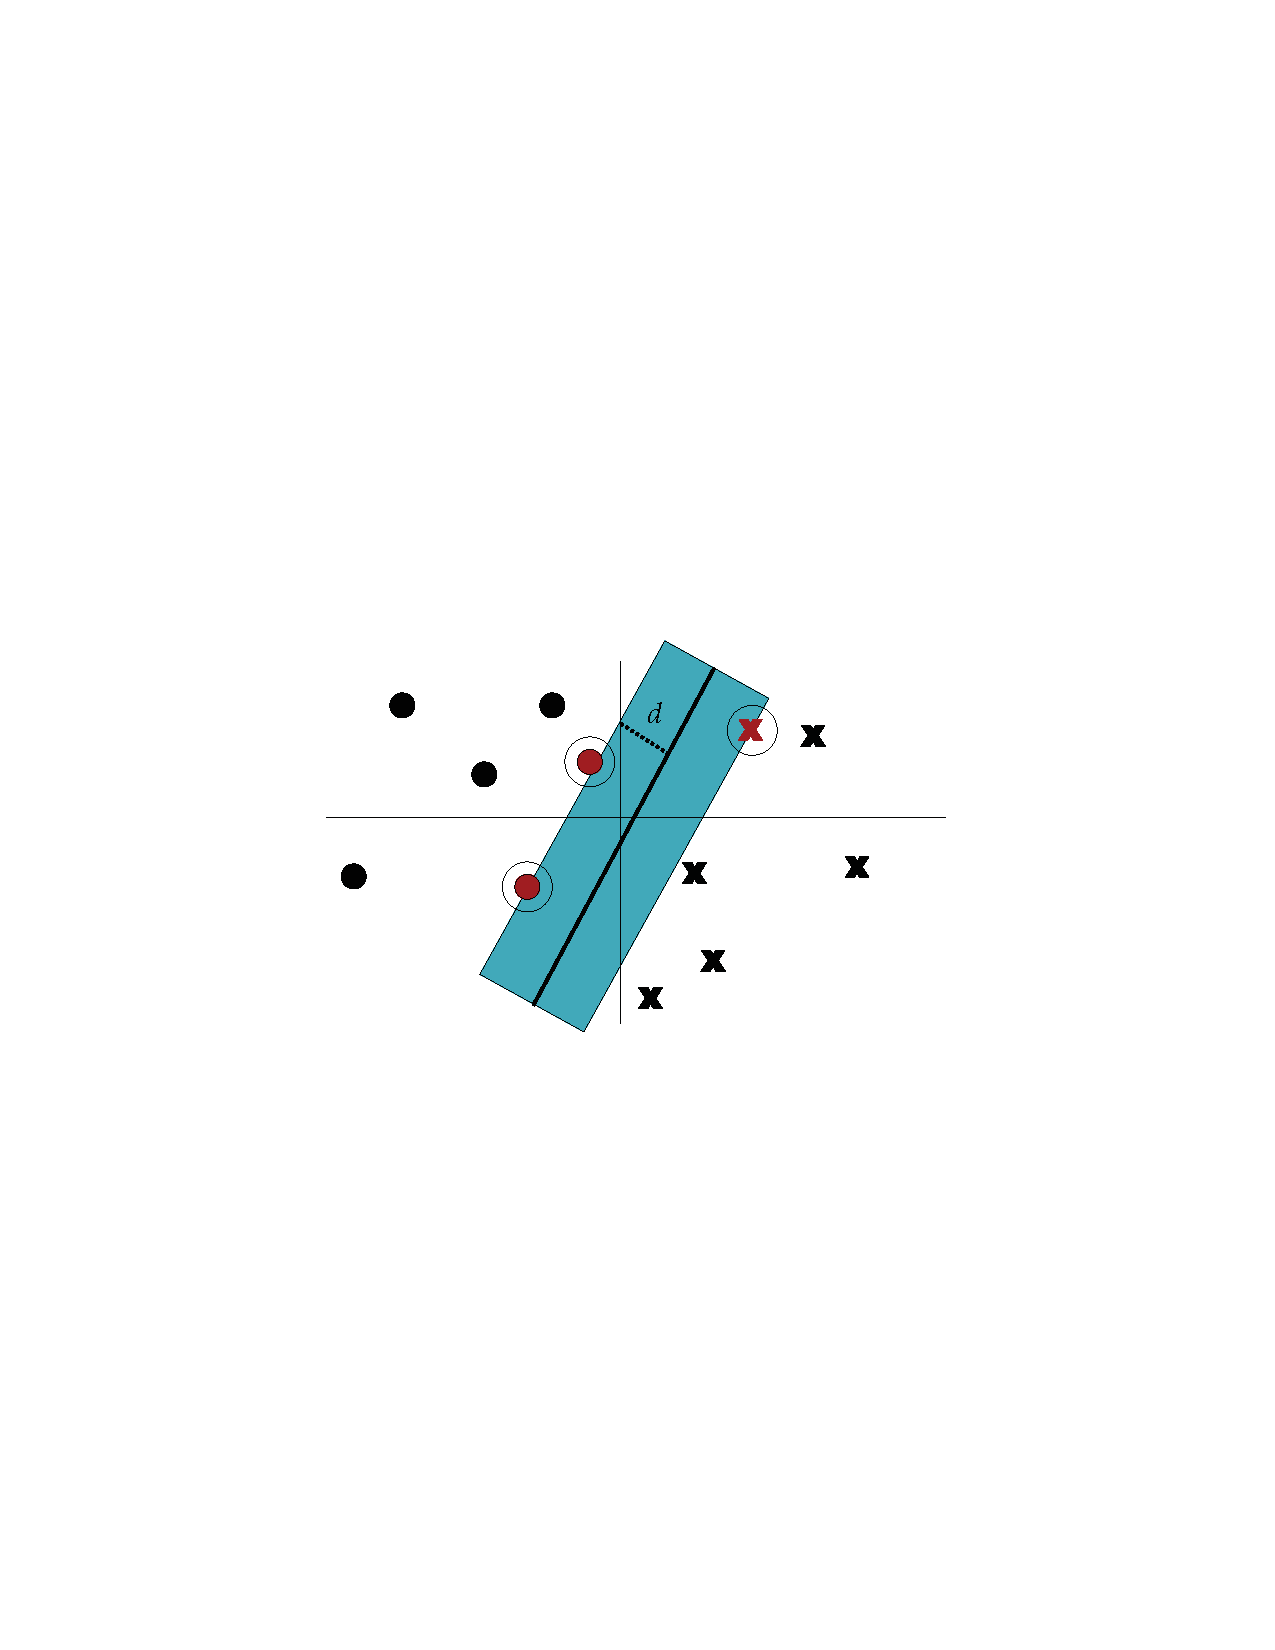
\includegraphics[width=0.6\textwidth]{figures/hyperplane}
  \caption{hyperplane}
  \label{fig:hyperplane}
\end{figure}

\subsection{K-Nearest Neighbor}

\subsection{Neural Networks}

\subsection{Ensemble Learning}
\label{subsec:ensemble_learning]}

\cite{ensemble2009Polikar}

\fi

\subsection{Deep Learning: Convolutional Neural Network}
\label{subsec:deep_learning}

In this section we will explain the fundamental of the algorithm on which the our solution is basen on, \acrlong{cnn}, a technology that was designed thinking mainly on computer vision tasks, but has proven to also for well on \acrshort{nlp} \cite{zhang2015sensitivity}, \cite{kim2014convolutional}. To understand how \acrshort{cnn} work, first we need to understand what a convolution is.

\section{Convolution}

A convolution could be defined as an integral that denotes the amount of overlap that the function $g$ shifts over another function $f$ (see figure \ref{fig:representation_convolution}).

Mathematically, a convolution is the product of two functions $f$ and $g$, depending on the values of the overlap are finite or not, the convolution (single dimension) could be defined as \cite{convolution}: 

\begin{figure}[!htp]
  \center
  \[[f \ast g](t)=\int_{0}^{t} f(\tau)g(t-\tau)d\tau\]
  \caption{Convolution for a finite range of $t \in [0, \infty]$}
  \label{fig:convolution_finite_range}
\end{figure}

or as:

\begin{figure}[!htp]
  \center
  \[f \ast g \equiv \int_{-\infty}^{\infty} f(\tau)g(t-\tau)d\tau\]\[=\int_{-\infty}^{\infty} g(\tau)f(t-\tau)d\tau\]
  \caption{Convolution for a infinite range of $t \in (-\infty, \infty)$}
  \label{fig:convolution_infinite_range}
\end{figure}

\begin{figure}[!htp]
  \center
  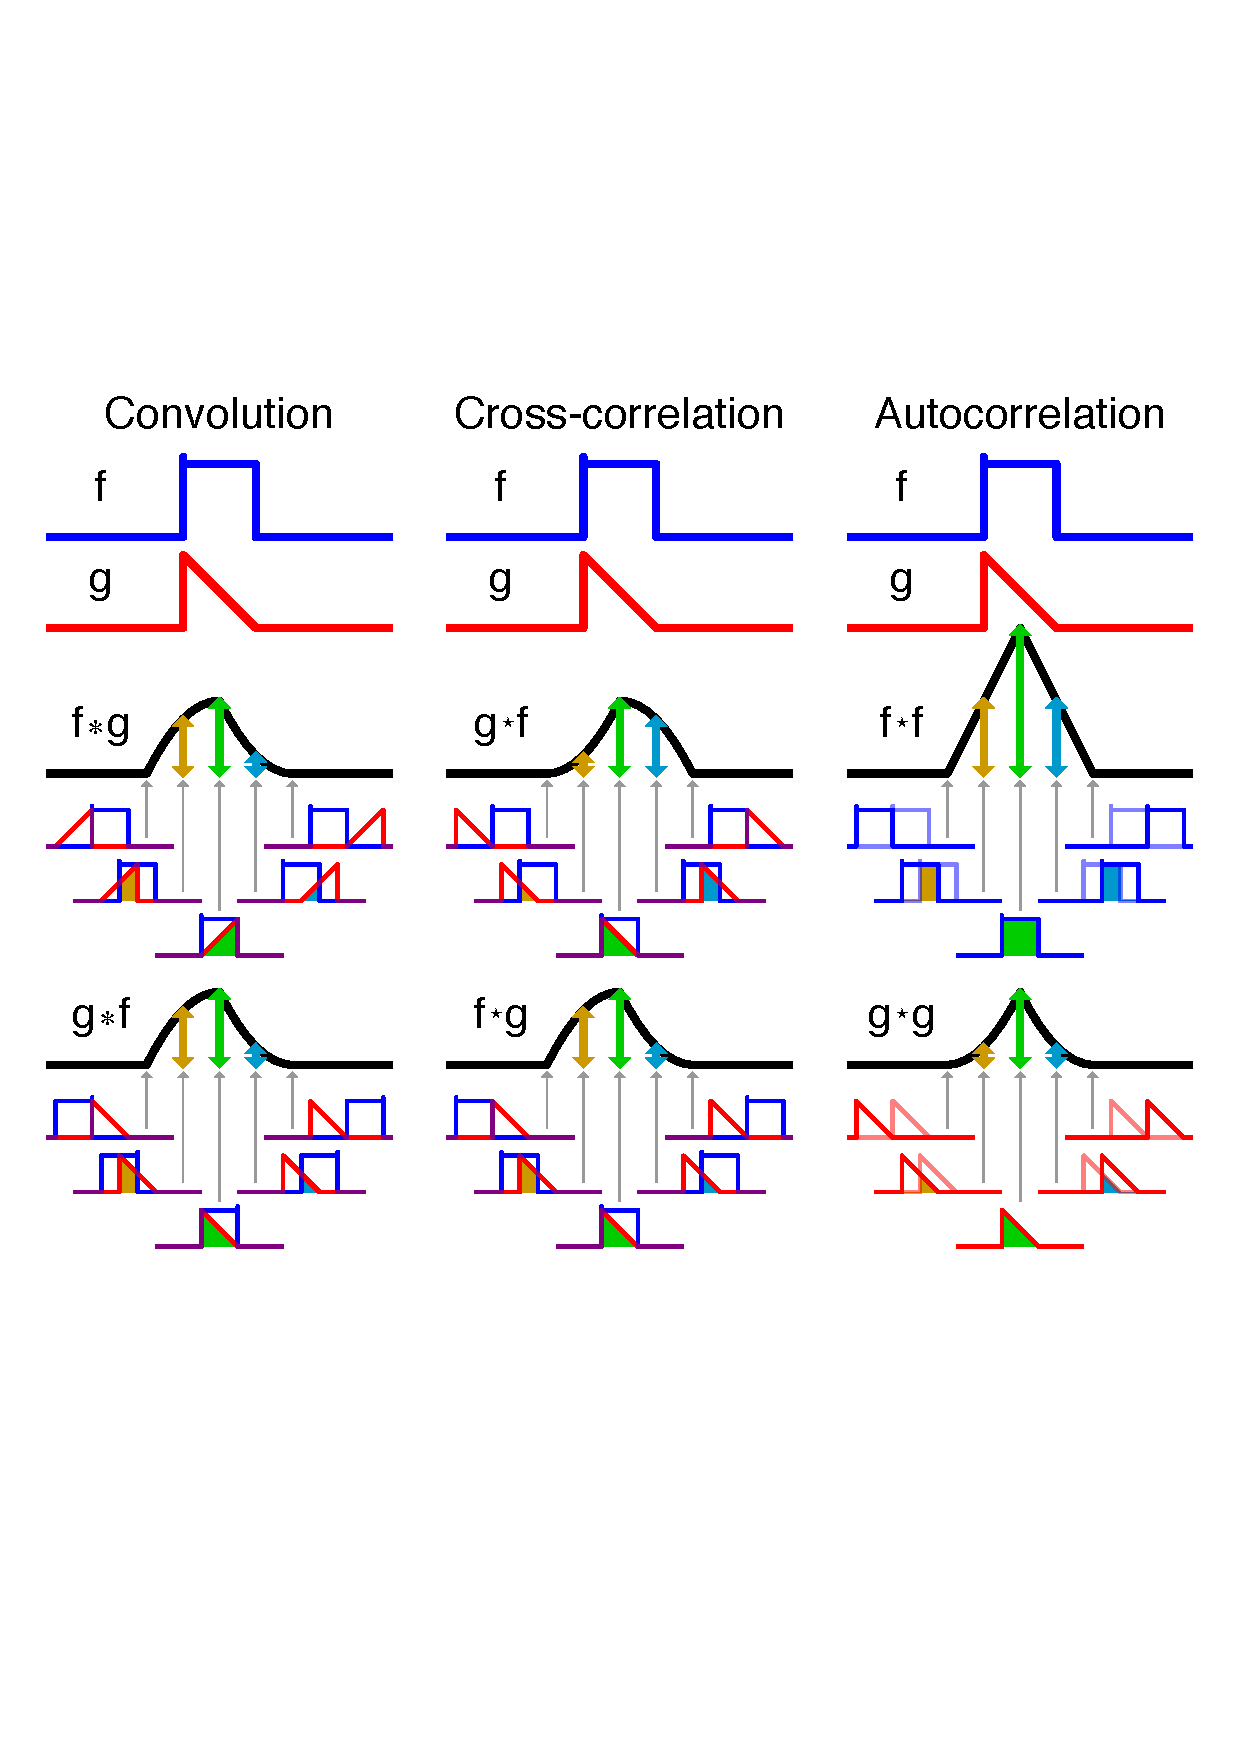
\includegraphics[width=0.6\textwidth]{figures/comparison_convolution_correlation}
  \caption{Graphical representation of a convolution and its comparison with correlation, image extracted from Wikipedia commons.}
  \label{fig:representation_convolution}
\end{figure}

A multidimensional convolution of infinite range the definition becomes \cite{multidimensionalConvolution}: 

\begin{figure}[!htp]
  \center
  \[f(t_1,t_2) \ast g(t_1,t_2) = \int_{t_1=-\infty}^{\infty}\int_{t_2=-\infty}^{\infty} f(\tau _1,\tau _2)g(t_1-\tau _1,t_2-\tau _2)d\tau _1 d\tau _2\]
  \caption{Multidimensional convolution for infinite ranges of $t_1,t_2 \in (-\infty, \infty)$}
  \label{fig:multidimension_convolution_infinite_range}
\end{figure}

In computer vision, images are transformed into two-dimensional functions, that can be represented as a matrix in which each value usually takes 0 or 1 values for black and white images or from 0 to 255 to gray-scale images. Most of the image transformation are based sliding window or function called ``kernel'', ``filter'' or ``feature detector'' \cite{cnnDennyBritz}, represented in figure \ref{fig:convolution_filter}.

\begin{figure}[!htp]
  \center
  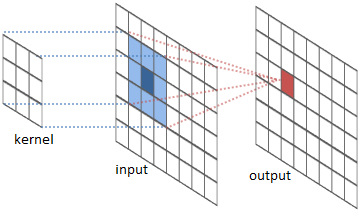
\includegraphics[width=0.6\textwidth]{figures/convolution_filter}
  \caption{Representation of a 2D image convolution transformation of filter size 3x3.}
  \label{fig:convolution_filter}
\end{figure}

\section{Convolutional Neural Networks}

\acrlong{cnn} are usually feed-forward type neural networks that concatenate multiple layers of convolutions with non linear activation functions as shown in figure \ref{fig:cnn_architecture}. The learning process of, for example, an image classification, learns the values by detecting the edges of the raw pixel values in the input of the \acrshort{cnn}. Over the following layers with the extraction of high level features, until reaching to last layer in which, all the fully connected layer classifies the objects by using the previously extracted features. 

\begin{figure}[!htp]
  \center
  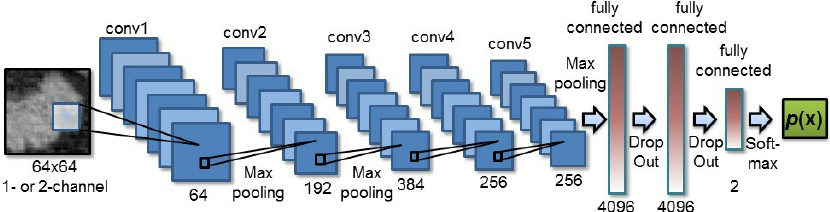
\includegraphics[width=0.96\textwidth]{figures/cnn_architecture}
  \caption{Example of a Convolutional Neural Network architecture \cite{kooi2017classifying}.}
  \label{fig:cnn_architecture}
\end{figure}

To apply the following architecture to \acrshort{nlp} related tasks, instead of a two convolution array that represents the image, each row of the matrix represents a token, usually being this tokens numerical representations of words or characters initialized with space vectors that are initialized with word2vec or GloVe algorithms. Then as with images each convolution layer extract features that are used on the last layer to categorize the given document as shown in figure \ref{fig:cnn_npl}. 

There are multiple types of architectures that combine multiple pooling layers that reduce computation cost by sub-sampling the matrix on each filter. In addition, as done in image processing, multiple channels of \acrshort{cnn} could be used to process each color, this idea can also translate into \acrshort{nlp} tasks by processing different word embeddings in each layer or applying different filters per channel \cite{singhalborrow}.

\begin{figure}[htbp]
  \center
  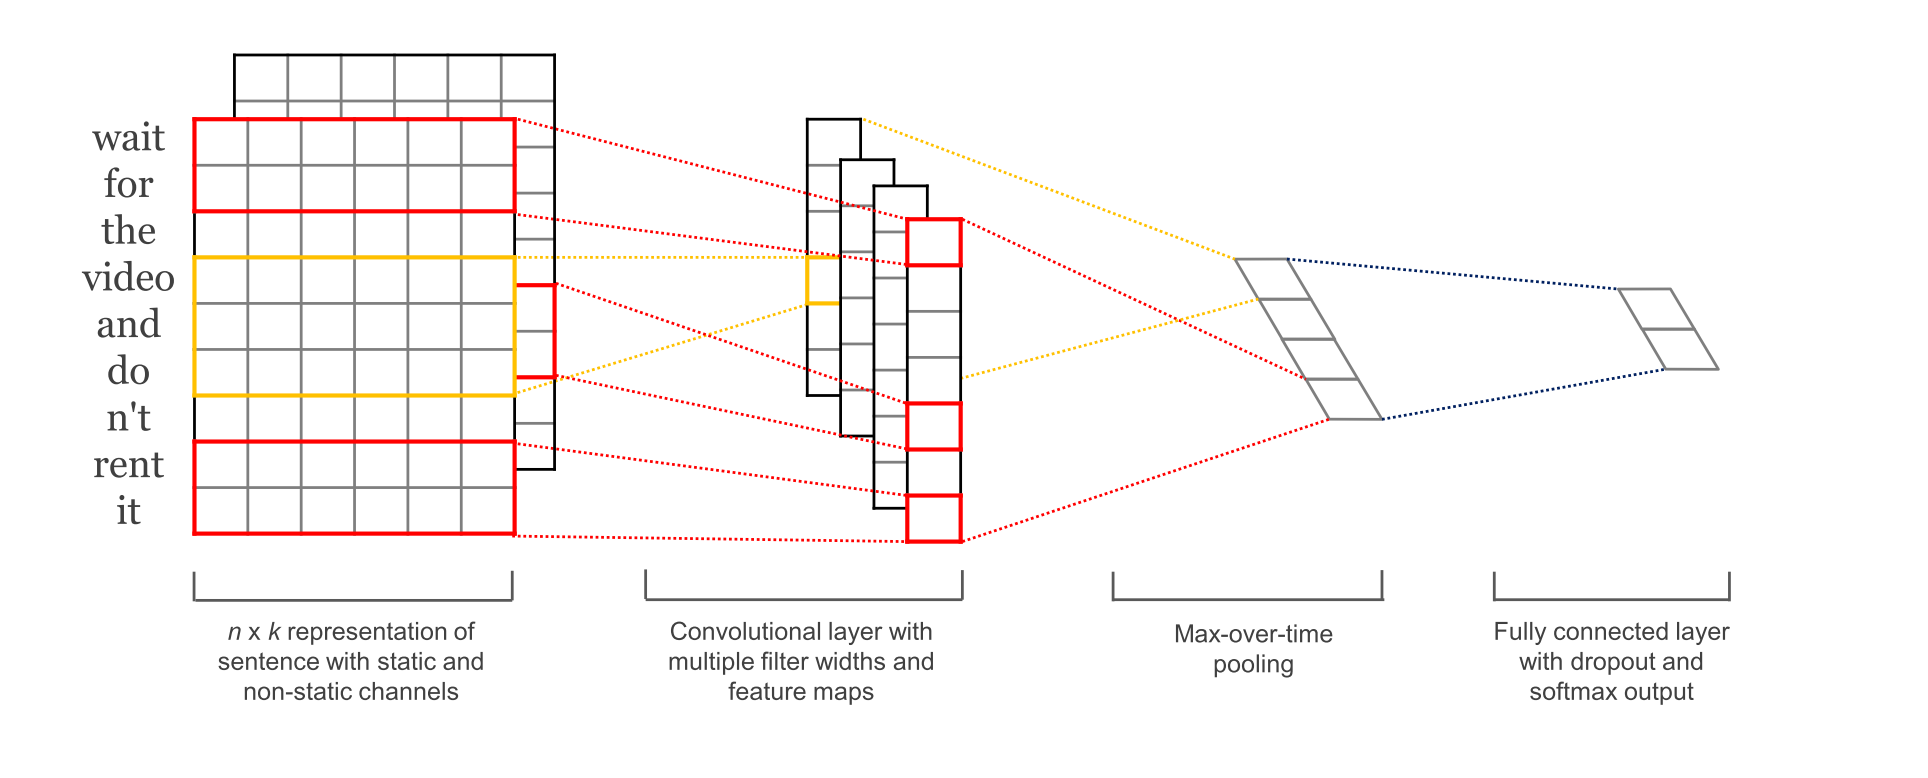
\includegraphics[width=0.7\textwidth]{figures/cnn_npl}
  \caption{Example of a Convolutional Neural Network architecture applied to NLP \cite{kim2014convolutional}.}
  \label{fig:cnn_npl}
\end{figure}
